% !TeX root = ../thuthesis-example.tex

\chapter{Kernel-level optimizations}\label{chapter-6}

\section{Fused-Experts Operator}
An essential factor to be able to run a Mixture-of-Experts model without incurring in great performance overhead is to use efficient GPU kernels. In particular, a MoE layer generally requires a fast implementation of a \textit{gating network}, \textit{top-k}, \textit{token dispatch}, \textit{expert prediction}, and \textit{predictions aggregation} kernel. In this section, we illustrate the role of each kernel, and how we implemented each of them in our \textit{fused-experts operator} in order to significantly optimize the performance when compared to the naive version.

\subsection{MoE-layer kernels}

\begin{algorithm}[H]
  \caption{Naive MoE-layer algorithm}
  \label{alg:naive-moe}
  \small
  \begin{algorithmic}[1]
    \Ensure $x$: input sequence, $W_{i}$: weights of expert $i \in [0, E)$, $GatingNetwork$: the weights of the FFN that implements the gating network, $k$: how many experts to route each token to, $E$: total number of experts, $C$: expert capacity, $seq\_len$: maximum number of tokens in each request, $batch\_size$: number of requests in each batch, $emb\_dim$: embedding dimension
    \Require shape of $x = [emb\_dim, seq\_len \cdot batch\_size]$
    \Require shape of $W_{i} = [emb\_dim, emb\_dim]$
    \Require $k \leq E$
    \State num\_tokens $\leftarrow$ seq\_len $\cdot$ batch\_size
    \State g $\leftarrow$ Softmax(GatingNetwork(x))
        \Comment{gating network kernel}
    \State top\_values, top\_indices $\leftarrow$ TopK(g)
        \Comment{top-k kernel}
    \State z $\leftarrow$ \Call{OneHotEncoding}{top\_indices, k, E, num\_tokens, C}
        \Comment{token dispatch kernel}
    \State predictions $\leftarrow$ x $\times$ z $\times \begin{bmatrix} W_0, \ \dots, \ W_{E-1} \end{bmatrix}^\top$
        \Comment{expert prediction kernel}
    \State output $\leftarrow$ dot(top\_values, predictions)
        \Comment{predictions aggregation kernel}
    \State 
    \Procedure{OneHotEncoding}{top\_indices, $k$, $E$, $num\_tokens$, $C$}
        \State Allocate a size of $k \cdot E \cdot num\_tokens $ for tensor $z$
        \State Allocate a size of $E$ for boolean array $num\_assignments$
        \State $z \leftarrow \{0\}$
        \State $num\_assignments \leftarrow \{0\}$
        \For{i}{0}{$num\_tokens$}
            \For{j}{0}{$k$}
                \State $e \leftarrow top\_indices[j,i]$
                \If{ $num\_assignments[e] \leq C$ }
                    \State $num\_assignments \leftarrow num\_assignments + 1$
                    \State $z[j,e,i] = 1$
                \EndIf
            \EndFor
        \EndFor
        \State return $z$
    \EndProcedure
  \end{algorithmic}
\end{algorithm}

Above, we present a naive algorithm (Algorithm \ref{alg:naive-moe}) to implement a MoE layer. In this version, we focus on the vanilla MoE model where each expert consists of a single fully-connected layer, and the gating network is also made up of a single fully-connected layer, followed by a softmax and a top-k. More realistic MoE layers will use more advanced components to achieve better load balancing, and improve the model's generalization power; for instance, several models~\cite{g-shard, original_moe}  add a stochastic components in the gating network. These additional components, however, are for the most part orthogonal to the issues we are discussing here, so we omit them for simplicity.

Each of lines 2-6 corresponds to one of the five typical MoE kernels introduced above. The algorithm should help demystifying what each such kernel does, and the dependencies between the kernels. We can implement Algorithm \ref{alg:naive-moe} in CUDA using a cuBLAS GEMM operator for the matrix multiplication steps, cuDNN for the softmax, and a custom CUDA kernel for the remaining steps. We can further implement a single fused kernel using CUDA or CUTLASS. However, the sparsity introduced by the one-hot encoding, together with the sequential nature of the two for loops (which are difficult to parallelize due to the need to consider the expert capacity when assigning tokens to experts) within the \textsc{OneHotEncoding} procedure lead the naive algorithm to suffer from poor performance in practice.

\subsection{\Project fast kernel implementation}
In \Project, we speed up the implement the \textit{token dispatch}, \textit{expert prediction}, and \textit{predictions aggregation} through the kernels shown below. In particular, Algorithm \ref{alg:moe-sort-tokens} allows us to parallelize the token dispatch operation, without exceeding the expert capacity. The kernel is carefully constructed so that each instruction is fully parallelizable. We take advantage of the Blelloch scan algorithm~\cite{blelloch_prefix_1990} to parallelize the \textit{reduction} and \textit{exclusive scan}, which would otherwise introduce a parallelization bottleneck. Each instruction in Algorithm \ref{alg:moe-sort-tokens} is implemented using the highly optimized NVIDIA Thrust library ~\cite{thrust}, which integrates seamlessly with the other kernels, which are written in CUDA. Thrust allows us to specify the execution policy for each instruction; by specifying the CUDA stream to use for each instruction, we can prevent any synchronization issue, while avoiding expensive operations such as \texttt{cudaDeviceSynchronize()}.

Algorithm \ref{alg:compute-batched-matmul-indices} illustrates our implementation of the \textsc{ComputeBatchedMatmulIndices} kernel, which takes the results of the \textsc{MoESortTokens} kernel as input, and populates three arrays of pointers that will then be used by the \textsc{BatchedMatmul} step (Algorithm \ref{alg:parallel-moe}, line 9) to compute the expert predictions, and one more array to be used in the final aggregation phase. Compared to the original naive algorithm, our design allows us to save GPU memory by not having to store the large one-hot encoding tensor. In addition, we remove most sparsity from the computations, resulting in better opportunities for speedups, since it is easier to optimize dense kernels. Finally, we perform most of our operations by manipulating the expert assignment indices, instead of the actual token data. This is beneficial because each index only requires one integer to represent, as opposed to the many floats required to represent each token, so we can save a lot of space and time. 

\begin{algorithm}[H]
  \caption{\textsc{MoESortTokens} kernel}
  \label{alg:moe-sort-tokens}
  \small
  \begin{algorithmic}[1]
    \Ensure $top\_indices$: the indices of the $k$ experts chosen by each token, $expert\_start\_idx$: the index of the first fused expert residing on the current device, $num\_experts\_per\_block$: number of fused experts residing on each device, $C$: expert capacity, $seq\_len$: maximum number of tokens in each request, $batch\_size$: number of requests in each batch
    \Require shape of $top\_indices = [k, seq\_len \cdot batch\_size]$    
    \Procedure{MoESortTokens}{top\_indices, expert\_start\_idx, num\_experts\_per\_block, C}
        \State num\_indices $\leftarrow$ length(num\_indices)
        \State original\_indices $\leftarrow$ sequence [ $0, \dots,  num\_indices -1 $ ]
        \State \textsc{StableSortByKey} (original\_indices, \textbf{key} = top\_indices)
        \State \textsc{StableSort} (top\_indices)
        \State lb\_index $\leftarrow$ \textsc{LowerBound} (top\_indices, \textbf{value} = expert\_start\_idx)
        \State ub\_index $\leftarrow$ \textsc{UpperBound} (top\_indices, \textbf{value} = expert\_start\_idx + num\_experts\_per\_block)
        \State num\_valid\_assignments $\leftarrow$ ub\_index - lb\_index
        \If{num\_valid\_assignments == 0}
            \State Done
        \EndIf
        \State nonzero\_expert\_labels, expert\_start\_indices $\leftarrow$ \textsc{Unique} ( top\_indices[ lb\_index : ub\_index ]  )
        \State nonzero\_expert\_count $\leftarrow$ length(nonzero\_expert\_labels)
        \State nonzero\_expert\_labels $\leftarrow$ nonzero\_expert\_labels - expert\_start\_idx
        \State temp\_sequence $\leftarrow$ sequence [ $0, \dots,  nonzero\_expert\_count -1 $ ]
        \State exp\_local\_label\_to\_index $\leftarrow$ \textsc{Scatter} (temp\_sequence, \textbf{map} = nonzero\_expert\_labels)
        \State expert\_start\_indices $\leftarrow$ \textsc{Append} (expert\_start\_indices, \textbf{value} = num\_valid\_assignments)
        \State expert\_start\_indices [1 : ] $\leftarrow$  expert\_start\_indices [1 : ] - expert\_start\_indices [ : -1]
        \State destination\_start\_indices $\leftarrow$ expert\_start\_indices [ : -1]
        \State destination\_start\_indices[destination\_start\_indices > C ] $\leftarrow$ C
        \State gemm\_batch\_count $\leftarrow$ \textsc{Reduce} (destination\_start\_indices)
        \State \textsc{ExclusiveScan} (destination\_start\_indices)
    \EndProcedure
  \end{algorithmic}
\end{algorithm}

\begin{algorithm}[H]
  \caption{\textsc{ComputeBatchedMatmulIndices} kernel}
  \label{alg:compute-batched-matmul-indices}
  \small
  \begin{algorithmic}[1]
    \Ensure $sorted\_indices$: the sorted indices of the $k$ experts chosen by each token
    \Ensure $original\_indices$ an array containing the reverse indices corresponding to the $sorted\_indices$
    \Ensure $exp\_local\_label\_to\_index$: a lookup table converting an expert label to its index
    \Ensure $expert\_start\_indexes$: the indices of the first tokens (in order) assigned to each unique expert in the block
    \Ensure $destination\_start\_indices$: the indices, for each expert, of the first slot in the index arrays belonging to each unique index
    \Ensure $input$: the tensor containing the input tokens
    \Ensure $weights$: tensor containing the weights for all the fused experts in the block
    \Ensure $coefficients$: tensor containing the $top\_values$ from the TopK operator
    \Ensure $output$: the output tensor
    \Ensure $num\_valid\_assignments$: the number of tokens who are assigned to experts in the current block
    \Ensure $lb\_index$: index of first slot in the $sorted\_indices$ tensor to belong to an expert in the block
    \Ensure $expert\_start\_idx$: the index of the first fused expert residing on the current device
    \Ensure $data\_dim$: embedding dimension of each token
    \Ensure $out\_dim$: hidden dimension of each output entry of the MoE layer
    \Ensure $C$: expert capacity
    \Ensure $k$: number of experts to which each token is assigned to
    
    \vspace{0.5cm}
    
    \Procedure{ComputeBatchedMatmulIndices}{sorted\_indices, original\_indices, exp\_local\_label\_to\_index, expert\_start\_indexes, destination\_start\_indices, input, weights, coefficients, output, num\_valid\_assignments, lb\_index, experts\_start\_idx, data\_dim, out\_dim, C, k}
    \State Allocate a size of $num\_valid\_assignments$ for each of pointer arrays  $token\_idx\_array$, $weight\_idx\_array$, $coefficient\_idx\_array$, and $output\_idx\_array$
    \State token\_idx\_array $\leftarrow \{0\}$
    \State weight\_idx\_array $\leftarrow \{0\}$
    \State coefficient\_idx\_array $\leftarrow \{0\}$
    \State output\_idx\_array $\leftarrow \{0\}$
        \ParallelFor{i}{0}{num\_valid\_assignments}
            \State global\_expert\_label $\leftarrow$ sorted\_indices[lb\_index + i]
            \State local\_expert\_label $\leftarrow$ global\_expert\_label - experts\_start\_idx
            \State expert\_index $\leftarrow$ exp\_local\_label\_to\_index[local\_expert\_label]
            \State within\_expert\_offset $\leftarrow$ i - expert\_start\_indexes[expert\_index]
            \State weight\_params\_count $\leftarrow$ data\_dim * out\_dim
            \If{within\_expert\_offset < C}
                \State rev\_idx $\leftarrow$ original\_indices[i + lb\_index]
                \State token\_idx $\leftarrow$ (rev\_idx / k)
                \State token\_idx\_array[destination\_start\_indices[expert\_index] + within\_expert\_offset] $\leftarrow$ \&input[token\_idx * data\_dim]
                \State weight\_idx\_array[destination\_start\_indices[expert\_index] + within\_expert\_offset] $\leftarrow$ \&weights[local\_expert\_label * weight\_params\_count]
                \State coefficient\_idx\_array[destination\_start\_indices[expert\_index] + within\_expert\_offset] $\leftarrow$ \&coefficients[rev\_idx]
                \State output\_idx\_array[destination\_start\_indices[expert\_index] + within\_expert\_offset] $\leftarrow$ \&output[token\_idx * out\_dim]
            \EndIf
        \EndParallelFor
    \State return $token\_idx\_array$, $weight\_idx\_array$, $coefficient\_idx\_array$, $output\_idx\_array$
    \EndProcedure
  \end{algorithmic}
\end{algorithm}



\begin{algorithm}[H]
  \caption{Fast algorithm for the MoE-layer}
  \label{alg:parallel-moe}
  \small
  \begin{algorithmic}[1]
    \Ensure $x$: input sequence, $W_{i}$: weights of expert $i \in [0, E)$, $GatingNetwork$: the weights of the FFN that implements the gating network, $k$: how many experts to route each token to, $E$: total number of experts, $C$: expert capacity, $seq\_len$: maximum number of tokens in each request, $batch\_size$: number of requests in each batch, $emb\_dim$: embedding dimension
    \Require shape of $x = [emb\_dim, seq\_len \cdot batch\_size]$
    \Require shape of $W_{i} = [emb\_dim, emb\_dim]$
    \Require $k \leq E$
    \State num\_tokens $\leftarrow$ seq\_len $\cdot$ batch\_size
    \State g $\leftarrow$ Softmax(GatingNetwork(x))
        \Comment{gating network kernel}
    \State top\_values, top\_indices $\leftarrow$ TopK(g)
        \Comment{top-k kernel}
    \State num\_experts\_per\_block $\leftarrow$ E / num\_devices
    \State sorted\_indices, original\_indices, exp\_local\_label\_to\_index, expert\_start\_indexes, destination\_start\_indices, num\_valid\_assignments, lb\_index $\leftarrow$ \Call{MoESortTokens}{top\_indices, expert\_start\_idx, num\_experts\_per\_block, C}
    \State experts\_start\_idx $\leftarrow device\_rank \cdot num\_experts\_per\_block$
    \State weights $\leftarrow \begin{bmatrix} W_0, \ \dots, \ W_{E-1} \end{bmatrix}^\top$
    \State token\_idx\_array, weight\_idx\_array, coefficient\_idx\_array, output\_idx\_array $\leftarrow$ \Call{ComputeBatchedMatmulIndices}{sorted\_indices, original\_indices, exp\_local\_label\_to\_index, expert\_start\_indexes, destination\_start\_indices, x, weights, coefficients, output, num\_valid\_assignments, lb\_index, experts\_start\_idx, emb\_dim, emb\_dim, C, k}
    \State predictions $\leftarrow$ \textsc{BatchedMatmul} (\textbf{a=}token\_idx\_array, \textbf{b=}weight\_idx\_array, \textbf{coeff=}coefficient\_idx\_array)
    \State \textsc{AtomicElementwiseAdd} (output\_idx\_array, predictions)

  \end{algorithmic}
\end{algorithm}


\section{Incremental Multi-Head Attention Kernel}

Our implementation of the Incremental Multi-head attention kernel closely follows Algorithm \ref{alg:attn2}, and is written in CUDA. We also make use of the cuBLAS and cuDNN libraries for operations such as matrix multiplications and activations, for which highly-optimized kernels available off-the-shelf are often faster than custom-designed ones. After designing algorithm \ref{alg:attn2}, an important aspect we considered during the implementation phase was how to effectively store all the data in memory, in such a way to simplify the access as much as possible. We designed the data layout in a way that minimizes the number of data copies and data movements needed, and we structured each tensor in column-major order, as is customary in CUDA. The layouts of the tensors used in the incremental multi-head attention layer are shown below:

\begin{figure}[H]
    \centering
    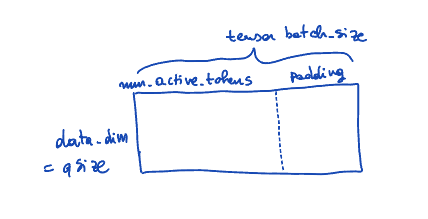
\includegraphics[width=0.6\linewidth]{figures/input_tensor.png}
    \caption{\textbf{The input tensor}}
    \label{fig:mha-input}
\end{figure}

\begin{figure}[H]
    \centering
    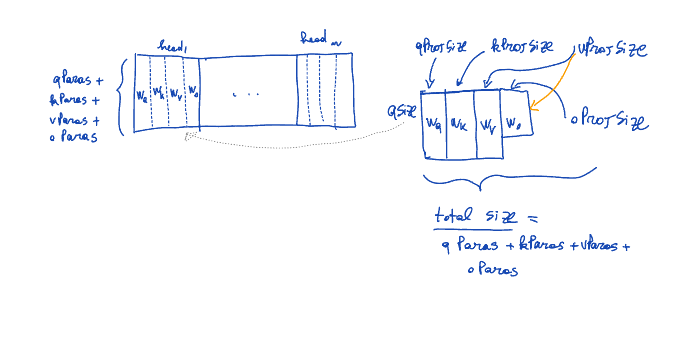
\includegraphics[width=\linewidth]{figures/weights.png}
    \caption{\textbf{The weights tensor}}
    \label{fig:mha-weights}
\end{figure}

\begin{figure}[H]
    \centering
    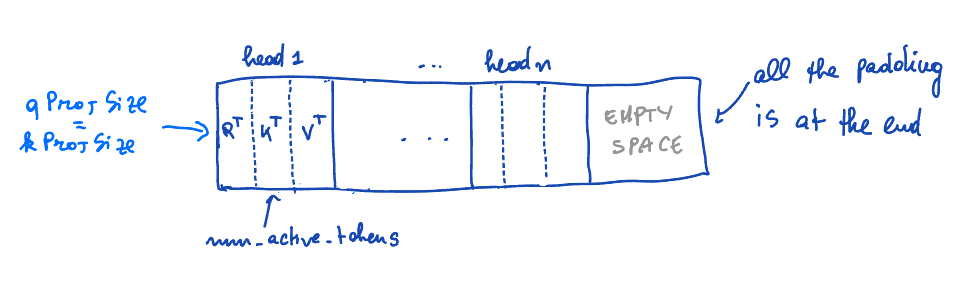
\includegraphics[width=\linewidth]{figures/qkv_proj.png}
    \caption{\textbf{The Q/K/V projections tensor}}
    \label{fig:mha-qkv-projs}
\end{figure}

\begin{figure}[H]
    \centering
    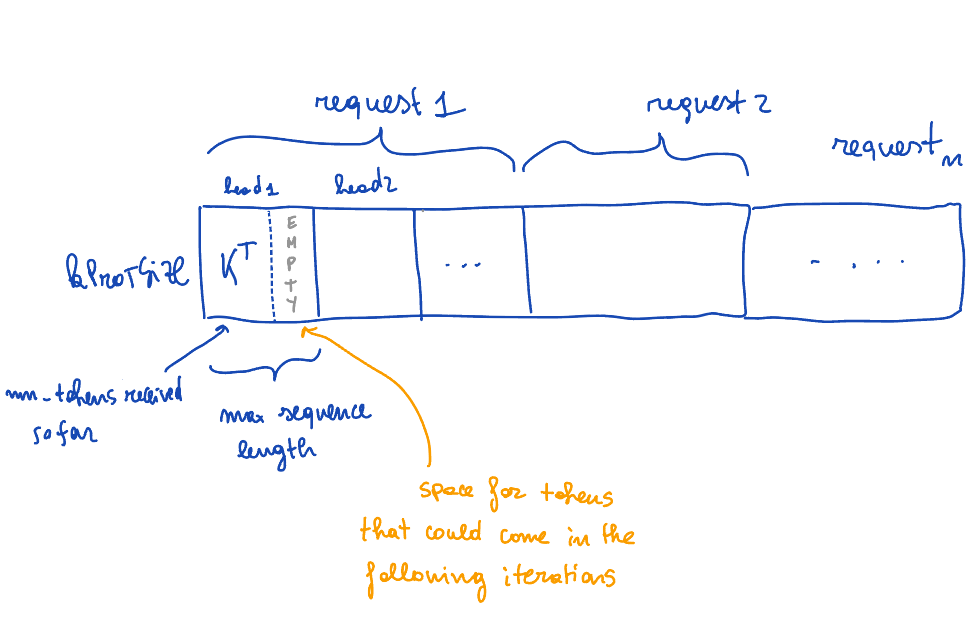
\includegraphics[width=\linewidth]{figures/kcache_tensor.png}
    \caption{\textbf{The K-cache tensor}}
    \label{fig:mha-kcache}
\end{figure}

\begin{figure}[H]
    \centering
    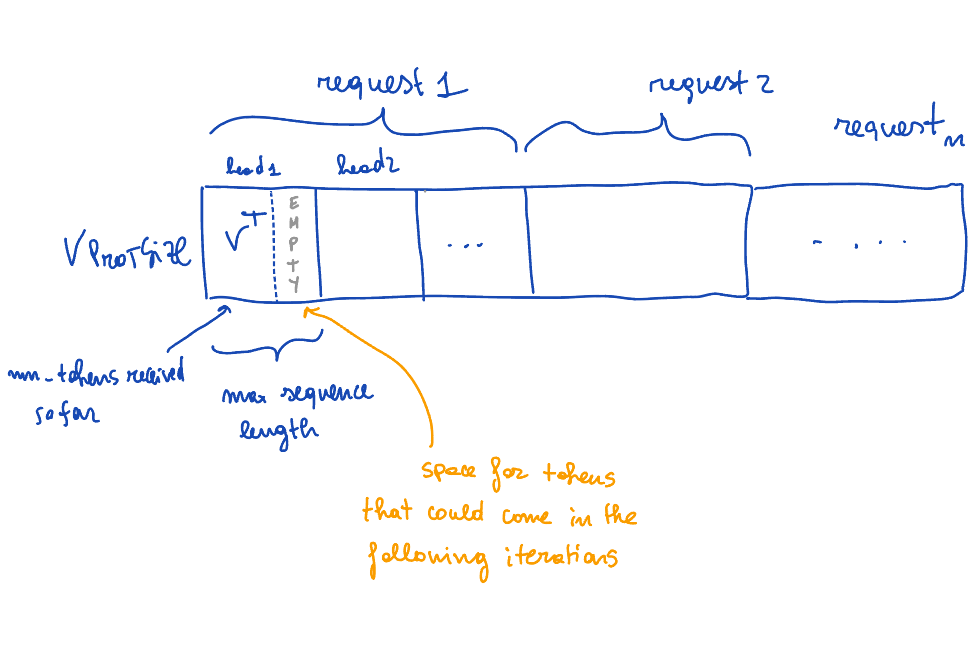
\includegraphics[width=\linewidth]{figures/vcache_tensor.png}
    \caption{\textbf{The V-cache tensor}}
    \label{fig:mha-vcache}
\end{figure}

\begin{figure}[H]
    \centering
    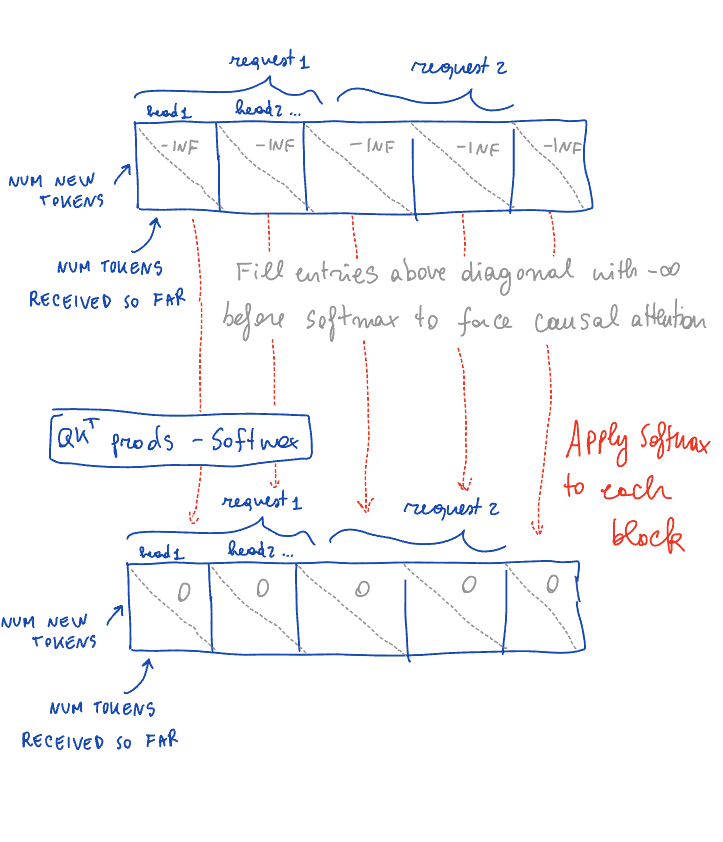
\includegraphics[width=\linewidth]{figures/qk_prods.png}
    \caption{\textbf{The QK-product tensor}}
    \label{fig:mha-qk-products}
\end{figure}

\begin{figure}[H]
    \centering
    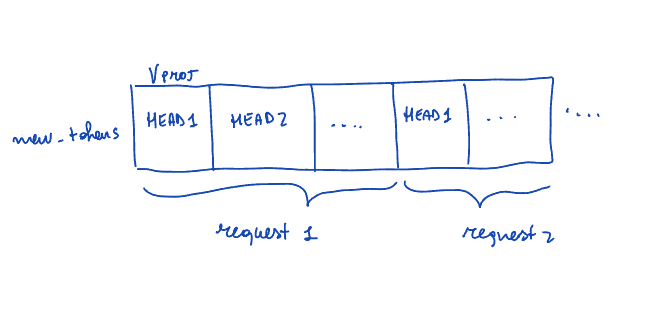
\includegraphics[width=0.6\linewidth]{figures/attn_heads.png}
    \caption{\textbf{The tensor containing the results for each attention head}}
    \label{fig:mha-attn-head}
\end{figure}

\begin{figure}[H]
    \centering
    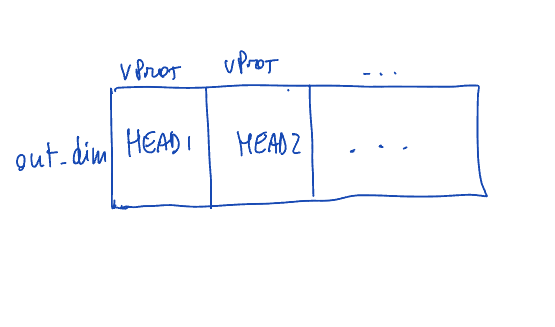
\includegraphics[width=0.6\linewidth]{figures/w_out-contiguous.png}
    \caption{\textbf{The output weights tensor}}
    \label{fig:w-out}
\end{figure}